\documentclass{article}

% if you need to pass options to natbib, use, e.g.:
%     \PassOptionsToPackage{numbers, compress}{natbib}
% before loading neurips_2018

% ready for submission
%\usepackage{neurips_2018}

% to compile a preprint version, e.g., for submission to arXiv, add add the
% [preprint] option:
\usepackage[preprint]{neurips_2018}

% to compile a camera-ready version, add the [final] option, e.g.:
%\usepackage[final]{neurips_2018}

% to avoid loading the natbib package, add option nonatbib:
%     \usepackage[nonatbib]{neurips_2018}

\usepackage[utf8]{inputenc} % allow utf-8 input
\usepackage[T1]{fontenc}    % use 8-bit T1 fonts
\usepackage{hyperref}       % hyperlinks
\usepackage{url}            % simple URL typesetting
\usepackage{booktabs}       % professional-quality tables
\usepackage{amsfonts}       % blackboard math symbols
\usepackage{nicefrac}       % compact symbols for 1/2, etc.
\usepackage{microtype}      % microtypography
\usepackage{epsfig}
\usepackage{graphicx}
\usepackage{xcolor}

\usepackage{amsfonts,amsmath,amssymb,amsthm}
\usepackage{bm,nicefrac}

\title{ECNet: Early Attention and Local Convolution for Machine Comprehension}

% The \author macro works with any number of authors. There are two commands
% used to separate the names and addresses of multiple authors: \And and \AND.
%
% Using \And between authors leaves it to LaTeX to determine where to break the
% lines. Using \AND forces a line break at that point. So, if LaTeX puts 3 of 4
% authors names on the first line, and the last on the second line, try using
% \AND instead of \And before the third author name.

\author{%
  %David S.~Hippocampus\thanks{Use footnote for providing further information
    %about author (webpage, alternative address)---\emph{not} for acknowledging
    %funding agencies.} \\
  %Department of Computer Science\\
  %Cranberry-Lemon University\\
  %Pittsburgh, PA 15213 \\
  %\texttt{hippo@cs.cranberry-lemon.edu} \\
	Abhishek Goswami\\
  Microsoft\\
  Redmond, WA 98052 \\
  \texttt{agoswami@microsoft.com} \\
  % examples of more authors
  % \And
  % Coauthor \\
  % Affiliation \\
  % Address \\
  % \texttt{email} \\
  % \AND
  % Coauthor \\
  % Affiliation \\
  % Address \\
  % \texttt{email} \\
  % \And
  % Coauthor \\
  % Affiliation \\
  % Address \\
  % \texttt{email} \\
  % \And
  % Coauthor \\
  % Affiliation \\
  % Address \\
  % \texttt{email} \\
}

\begin{document}
% \nipsfinalcopy is no longer used

\maketitle

\begin{abstract}

Current state-of-the-art machine comprehension models have two common tenets. One, use of an embedding encoder layer over the  input embeddings to exploit contextual cues from surrounding words. Two, use of neural attention mechanisms over the context and query to exploit the notion of matching. In this paper we propose ECNet, a hierarchical model for machine comprehension, which amplifies existing models by adding early attention and local convolution. It uses self-attention over the input embeddings as a form of early attention. For the embedding encoder layer, it models both sequential and local interactions between words, using recurrent and convolution layers respectively.  On the SQuAD 2.0 dataset, ECNet outperforms the BiDAF model proposed recently in literature

\end{abstract}

\section{Introduction}
\label{sec:introduction}

For the final project of CS224n, we chose to do the default project. We also propose a slight variant of this problem as a strech goal (Section \ref{subsec:projectstrechgoals}) where we would like some feedback on the proposed idea.

The author is a SCPD student in a single person team. There are no external collaborators. We are looking forward to a mentor being assigned to us, since we have no particular mentor. We are are not sharing this project with any other class.


\section{Model}
\label{sec:model}

In this section, we first formulate the machine comprehension problem and then describe the model. 

\subsection{Problem Statement}
\label{subsec:problemstatement}

The machine comprehension task considered in this paper is as follows. Given a context paragraph with $T$ words, C = \{$c_1$, $c_2$, ..., $c_T$\} and a query sentence with $J$ words, Q = \{$q_1$, $q_2$, ... $q_J$\}, output a span S = \{$c_i$, $c_{i+1}$,...${c_{i+j}}$\} from the original paragraph C that satisfactorily answers the question. Section ~\ref{subsec:metricdetails} describes two metrics that are widely used in literature for evaluating this task. We use $d$ to represent the hidden size used by several layers of the model.

\begin{table}[htbp]
    \caption{An example of a machine comprehension task.}
    \label{table:economicSchools} 
    \centering
    \begin{tabular}{|l|p{0.8\linewidth}|}
    \hline
    Question   &  Economy, Energy and Tourism is one of the what? \tabularnewline \hline
    Context  & Subject Committees are established at the beginning of each parliamentary session, and again the members on each committee reflect the balance of parties across Parliament. Typically each committee corresponds with one (or more) of the departments (or ministries) of the Scottish Government. The \textcolor{blue}{current Subject Committees} in the fourth Session are: Economy, Energy and Tourism; Education and Culture; Health and Sport; Justice; Local Government and Regeneration; Rural Affairs, Climate Change and Environment; Welfare Reform; and Infrastructure and Capital Investment \tabularnewline \hline
    Answer   & current Subject Committees \tabularnewline \hline
    \end{tabular}
 
\end{table}

\subsection{Model Overview}
\label{subsec:models}

Several state-of-the-art machine comprehension models have a similar structure. They have (a) an embedding layer (b) an embedding encoder layer (c) an attention flow layer (d) a model encoder layer and (e) an output layer. 

We introduce two novel extensions to this structure.  One, we add a Embedding Attention Layer between the input Embedding Layer and the Embedding Encoder Layer, with the goal of introducing early attention in the modeling process. Second, for the Embedding Encoder Layer we use a combination of recurrent and convolution operations to make it rich with both sequential and local interactions. Our machine comprehension model is thus a hierarchical multi-stage process consisting of six layers. 

\begin{enumerate}
\item Embedding Layer. 
\item Embedding Attention Layer.
\item Embedding Encoder Layer.
\item Attention Flow Layer.
\item Model Encoder Layer.
\item Output Layer.
\end{enumerate}

\begin{figure*}[h!]
\centering
	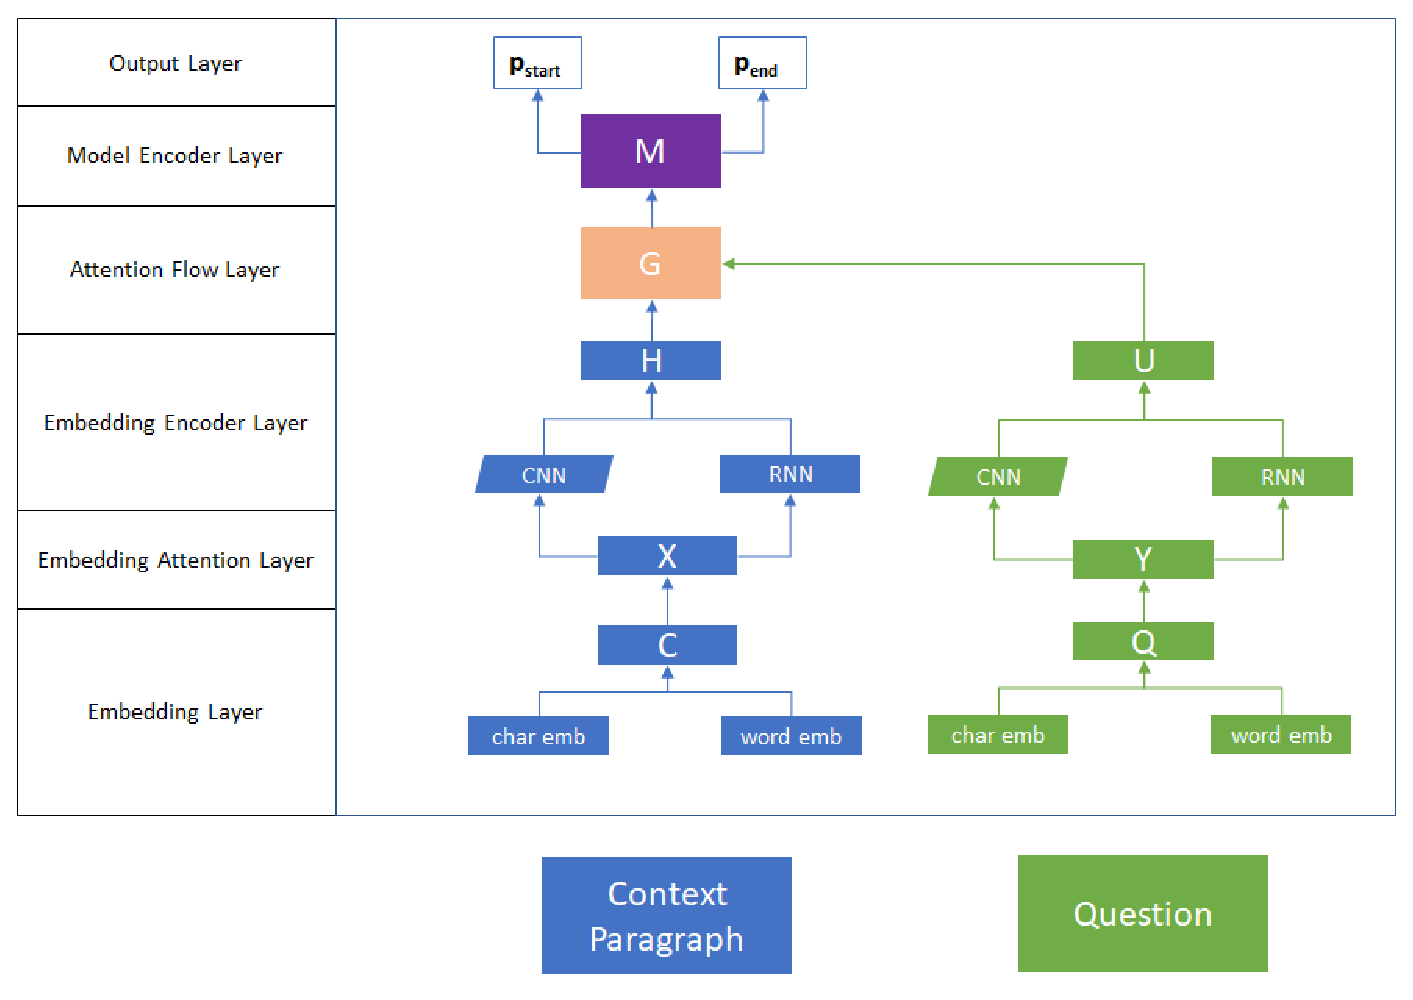
\includegraphics[width=12cm]{Figs4Paper/Model2.eps}
  \caption{Model architecture}
  \label{fig:modelarchitecture}
\end{figure*}

The details of each of the layers are as follows.

\paragraph{1. Embedding Layer.} In this layer we mix character embeddings with word embeddings. 

For character embeddings, we use a method similar to that proposed by Kim et al \cite{kim2016character}. We first convert a word to its character indices. We then pad (or truncate) each word so it has length $m_{word}$.  For each of these characters we lookup a dense character embedding (which has shape ${e_{char}}$). To combine the character embeddings, we use 1-dimensional convolutions over $m_{word}$ using ${e_{char}}$ as the input channel size and ${e_{word}}$ as the output channel size. The output of the CNN are max-pooled over the entire width to obtain a fixed-size vector of shape ${e_{word}}$ for each word. 

For word embeddings, we use pre-trained word vectors from GloVe \cite{pennington2014glove} to obtain the fixed embedding for each word. The size of the word embeddings is ${e_{word}}$ which is the same as the shape of the character-level embeddings for each word.  

The concatenation of the character and word embeddings is passed to a Highway Network \cite{srivastava2015highway}. We do this for both the context sentence $C$ and also the question $Q$. So now we have two matrices \textbf{C} $\in \mathbb{R}^{T, d}$  and \textbf{Q} $\in \mathbb{R}^{J, d}$ corresponding to the context and question respectively.

\paragraph{2. Embedding Attention Layer.} The motivation for adding this layer is to attend to the embeddings provided by the previous layer. This layer starts early attention to the word and character character embeddings. As before, we do this for both the context sentence $C$ and also the question $Q$ , and concatenate the results with the embedding layer output giving us two matrices \textbf{X} $\in \mathbb{R}^{T, 2d}$  and \textbf{Y} $\in \mathbb{R}^{J, 2d}$ corresponding to the context and question respectively. 

\paragraph{3. Embedding Encoder Layer.} The purpose of this layer is to encode the relationships between the embeddings provided by the previous layers. On one hand we want to model the temporal interactions between words. For this we use a bi-directional LSTM. This results in two matrices of shape $(T, 2d)$ and $(J, 2d)$ corresponding to the context and question respectively. 

We also model local interactions between the embeddings output by the embedding attention layer. We use 1-dimensional convolutions over the sequence length using $2d$ as both the input and output  channel size. We do this using a kernel size 1,  which results in two matrices of shape $(T, 2d)$ and $(J, 2d)$ corresponding to the context and question respectively. 

The concatenation of the RNN and CNN layers gives us two matrices \textbf{H} $\in \mathbb{R}^{T, 4d}$ and \textbf{U} $\in \mathbb{R}^{J, 4d}$ respectively.   

\paragraph{4. Attention Flow Layer.} We also add a bi-directional attentional flow layer introduced by Seo et al \cite{seo2016bidirectional}. The main idea is that attention should flow both ways - from the context to the question and from the question to the context. The attention flow layer also fuses the information between the context and the query words. 

The inputs to the layer are contextual vector representations of the context \textbf{H} and the query \textbf{U}. The outputs of the layer is \textbf{G} $\in \mathbb{R}^{T, 16d}$ which is a query-aware vector representations of the context words, along with the embeddings from the previous layer.
 
\paragraph{5. Model Encoder Layer.} This layer encodes the query-aware representations of the context words. The input is \textbf{G}, and the output is matrix \textbf{M}, which captures the interaction among the context words conditioned on the query. We use two layers of bi-directional LSTM, with hidden size $d$ for each direction. Matrix \textbf{M} $\in \mathbb{R}^{T, 2d}$  is then passed to the Output Layer. 

\paragraph{6. Output Layer.} This layer is application specific.  For the QA task being explored in this project, we need to find a sub-phrase of the context to answer the query. The phrase is derived by predicting the start and end indices of the phrase in the paragraph. 
The output layer produces two probability distribution $\bm{p}_{start}$, $\bm{p}_{end}$  $\in \mathbb{R}^N$ corresponding to each position in the context. 

\begin{equation}
\bm{p}_{start} = \text{softmax}(\bm{W}_{start}[\bm{G}; \bm{M}]).
\end{equation}

\begin{equation}
\bm{p}_{end} = \text{softmax}(\bm{W}_{end}[\bm{G}; \bm{M'}]).
\end{equation}

where $\bm{M'}$  $\in \mathbb{R}^{T, 2d}$ is a matrix obtained by applying a bi-directional LSTM to $\bm{M}$.


%\begin{figure*}[h!]
%\centering
	%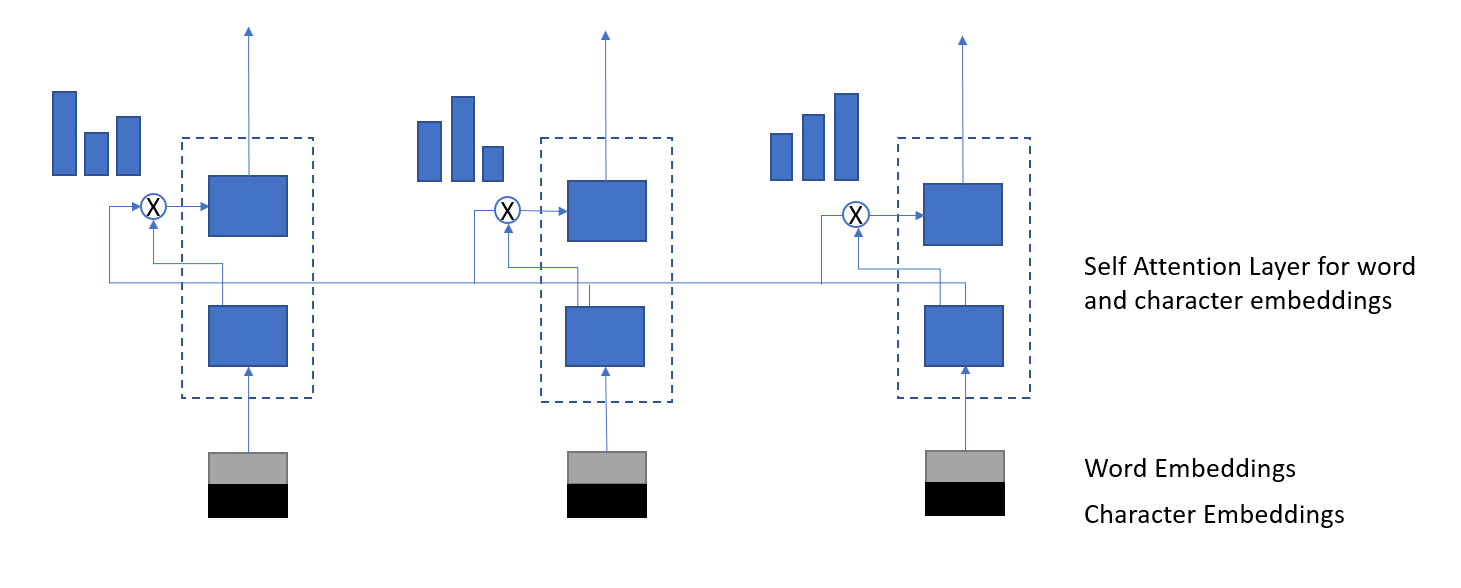
\includegraphics[width=12cm]{Figs4Paper/EarlyAttentionLayer.eps}
  %\caption{Convolutional network architecture}
  %\label{fig:convnetarchitecture}
%\end{figure*}
 
\subsection{Model Training and Scoring}
\label{subsec:modeltrainingandscoring}

\paragraph{Training.} We define the training loss as the sum of the negative log-likelihood (cross-entropy) loss for the start and end locations. So for a (context, question) pair with \textit{start} index {i} $\in \{1, 2, ..., T\}$ and \textit{end} index {j} $\in \{1, 2, ..., T\}$

\begin{equation}
\text{loss} = - \text{log} \, \bm{p}_{start}(i) - \text{log} \, \bm{p}_{end}(j).
\end{equation}

During training, we average across the batch and use the Adadelta optimizer \cite{zeiler2012adadelta} to minimize the loss.

\paragraph{Scoring.} At test time, we chose the pair (i,j) of indices that maximizes $\bm{p}_{start}(i).\bm{p}_{end}(j)$ subject to $i \leq j$ and $j - i + 1 \leq L_{max}$, where $L_{max}$ is a hyperparameter which sets the maximum length of a predicted answer.  

\paragraph{No Answer.}  We adopt the approach proposed by Levy et al \cite{levy2017zero}. We prepend a OOV token to the beginning of each sequence. The model outputs $\bm{p}_{start}$ and $\bm{p}_{end}$ soft-predictions as usual. When discretizing a prediction, if $\bm{p}_{start}(0)$· $\bm{p}_{end}(0)$ is greater than any predicted answer span, the model predicts no-answer. Otherwise the model predicts the highest probability span. Note, this approach also allows us to predict a per-example confidence score that the question is unanswerable.
\section{Experiment}
\label{sec:experiment}

In this section, we conduct experiments to study the performance of our models. We will benchmark our models on the Stanford Question Answering Dataset (SQuAD) 2.0 \cite{rajpurkar2018know}, considered to be one of the most competitive datasets in QA tasks. We also provide some implementation details for our models and present the main results.

\subsection{Dataset}
\label{subsec:dataset}

We consider the Stanford Question Answering Dataset (SQuAD) 2.0 \cite{rajpurkar2018know} for machine comprehension. Our model is given a paragraph, and a question about that paragraph, as input. The goal is to answer the question correctly. There are around 150k questions, and roughly half of the questions cannot be answered using the provided paragraph. 


\subsubsection{Data splits}
\label{subsubsec:dataset}

The official SQuAD dataset has three splits: train, dev and test. The train and dev sets are publicly available and the test set is entirely secret. For this project we use a custom dev and test set obtained by splitting the official dev set in half. 

To summarize we have the following data splits:

\begin{itemize}
\item \textbf{Train}. 129,941 examples. All taken from the official SQuAD 2.0 training set.
\item \textbf{Dev}. 6,078 examples. Roughly half of the official dev set, randomly selected.
\item \textbf{Test}. 5,915 examples. The remaining examples from the official dev set.
\end{itemize}

From now on we refer to these splits as the train set, dev set and test set respectively. We will use the train set to train the model. We report the performance metrics on the dev set.

\subsection{Training Details}
\label{subsec:trainingdetails}

The model architecture used for this task is shown in Figure \ref{fig:modelarchitecture}. 

For the Embedding Layer, $m_{word}$ is set to 16. ${e_{char}}$ and ${e_{word}}$ are set to 64 and 300 respectively. We use one 1D filter for the CNN char embedding with a kernel size of 5. The hidden state $d$ of the model is 100. For the convolutions in the Embedding Encoder Layer, we use a set of 4 stacked CNN layers, each with input/output channels as $2d$ with a kernel size of 1 . We uses dropout as a form of regularization across all the six layers in our model. Table \ref{table:dropoutresults} shows the effect of dropout on our model performance. We use the Adadelta optimizer \cite{zeiler2012adadelta} with a learning rate of 0.5 which is kept fixed. While training we use a batch size of 64. When scoring, $L_{max}$ is set to 15.

We implement our model in Python using PyTorch \cite{pytorch}. The experiments are carried out on a Azure Data Science Virtual Machine (DSVM) \cite{dsvm} which has a NVIDIA Tesla K80 GPU.

\subsection{Metric Details}
\label{subsec:metricdetails}

We measure performance via two metrics: Exact Match (EM) and the F1 score.

\begin{itemize}
\item \textbf{Exact Match} is a binary measure (i.e. true/false) of whether the system output matches the ground truth answer exactly.
\item \textbf{F1} is the harmonic mean of precision and recall.
\item When a question has no answer, both the F1 and EM score are 1 if the model predicts no-answer, and 0 otherwise.
\item For questions that do have answers, when evaluating on the dev or test sets, we take the maximum F1 and EM scores across the three human-provided answers for that question.
\end{itemize}

\subsection{Results}
\label{subsec:results}

\begin{figure*}[h!]
\centering
	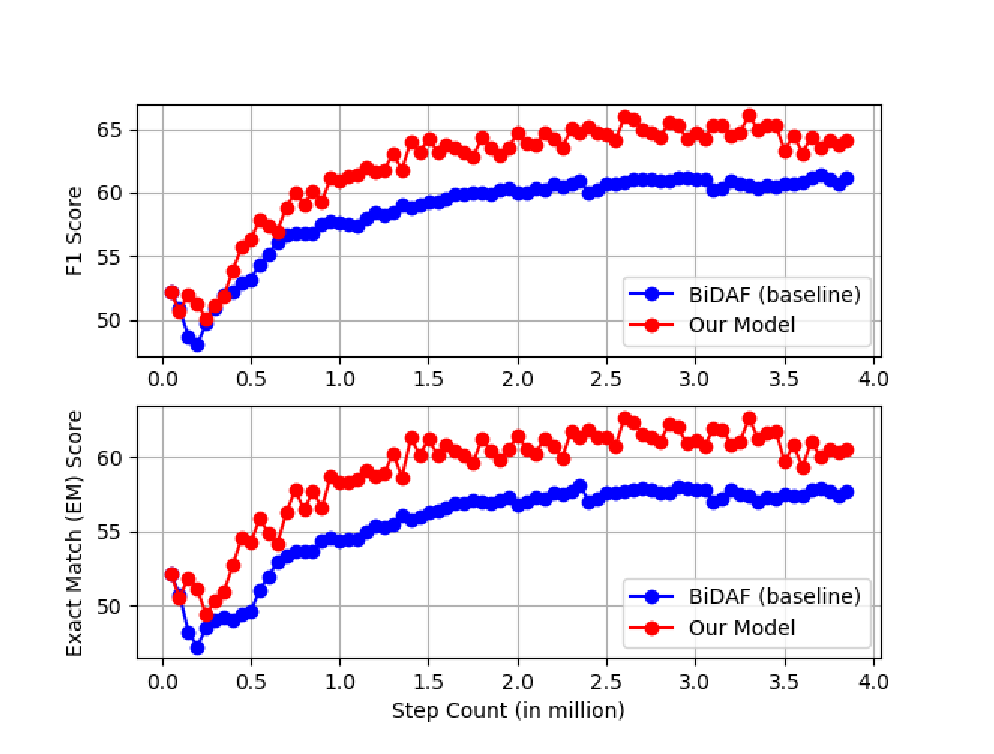
\includegraphics[width=12cm]{Figs4Paper/F1EM.eps}
  \caption{Comparison of F1 and EM scores}
  \label{fig:f1em}
\end{figure*}


\begin{table}[]
\caption{Comparing our model with the baseline}
\label{table:results}
\centering
\begin{tabular}{lll}
																									& EM    & F1    \\ \hline
BiDAF with character embedding (baseline)				  & 59.47 & 62.46 \\
Our Model																					& 62.64 & 66.10 \\ \hline

\end{tabular}
\end{table}

Table \ref{table:results} shows the comparison between our model and the baseline. As per the original BiDAF model, we include a character-level embedding layer using character-level convnets. This gives us a very strong baseline to compare with.


\subsection{Ablations}
\label{subsec:ablations}


\begin{table}[]
\caption{Results from Ablation Study}
\label{table:ablation}
\centering
\begin{tabular}{lll}
                                                                       & EM    & F1    \\ \hline
No Embedding Attention Layer                                           & 60.93 & 64.34 \\
No CNN layers inside the Embedding Encoder Layer                       & 59.64 & 63.10 \\
No character embedding in the Embedding Layer                          & 59.47 & 62.46 \\
Freezing both the character and word embeddings in the Embedding Layer & 62.19 & 65.39 \\ \hline

\end{tabular}
\end{table}


Table \ref{table:ablation} shows the performance of the model and its ablations on the SQuAD dev set. Having an Embedding Attention Layer helps model performance. This validates our hypothesis that adding attention layers early in the model stack should help performance. For ablating the effect of the CNN layers, we experiment by removing the CNN layers from the Embedding Encoder Layer. CNN layers prove to be critical with a drop of 3 points on both metrics. As noted by Seo at al \cite{seo2016bidirectional}, having character embeddings in the Embedding Layer contributes towards model performance whereby word-level embeddings represent the semantics of each word as a whole, while char-level embeddings better handle out-of-vocab (OOV) or rare words. Interestingly we also see that freezing the char-level and word-level embeddings gives us slightly lower performance. It seems the model gives slightly better results if we allow the backpropagation to happen all the way through the embedding layer, and the fine-tuned embeddings generalize quite well to unseen data in the dev set. 

\begin{table}[]
\caption{Effect of dropoput}
\label{table:dropoutresults}
\centering
\begin{tabular}{lll}
																	& EM    & F1    \\ \hline
No Dropout		   									& 60.41 & 63.46 \\
Dropout = 0.1    									& 62.06 & 65.39 \\ 
Dropout = 0.2 (chosen)		  			& 62.64 & 66.10 \\ 
Dropout = 0.3    									& 59.84 & 63.81 \\ 
Dropout = 0.4    									& 61.10 & 64.09 \\ \hline

\end{tabular}
\end{table}

Table \ref{table:ablation} shows the effect of dropout rates. With low dropout rates, the model was overfitting.  High drop-out rates help in preventing overfitting, but lead to lower EM/F1 scores. We settle on 0.2 as the dropout rate since it gave the best results.

% -----------------------------------------------
%\subsection{Implementation Details}
%\label{subsec:implementationdetails}

\begin{table}[]

    \caption{Preliminary Results}
    \label{table:results} 
    \centering
		
\begin{tabular}{|l|l|l|l|l|}
\hline
                                                                & \multicolumn{2}{l|}{\textbf{Dev Set}} & \multicolumn{2}{l|}{\textbf{Test Set}} \\ \hline
                                                                & EM                & F1                & EM                 & F1                \\ \hline
master                        				                          & 59.25             & 62.28             & 59.47              & 62.46             \\ \hline
baselinemodel\_selfsimilaritybeforeattention								 		& 58.83             & 62.05             & 57.47              & 60.87             \\ \hline
baselinemodel\_selfsimilarityafterattention								 			& 59.45             & 62.95             & 59.45              & 62.95             \\ \hline
conflict\_without\_for\_loops																 		& 55.67             & 59.19             & 55.67              & 59.19             \\ \hline
embedding\_with\_self\_similarity                               & 59.64             & 63.10             & 59.64              & 63.10             \\ \hline
embedding\_with\_self\_difference                               & 52.19             & 52.19             & 52.19              & 52.19             \\ \hline
conv\_rnn\_embed\_layer							                  	        & 60.93             & 64.34             & 60.93              & 64.34             \\ \hline
embedding\_with\_self\_similarity\_conv\_rnn (0.0)              & 62.19             & 65.26             & 60.41              & 63.46             \\ \hline
embedding\_with\_self\_similarity\_conv\_rnn (0.1)              & 62.19             & 65.26             & 62.06              & 65.39             \\ \hline
embedding\_with\_self\_similarity\_conv\_rnn (0.2)              & 62.19             & 65.26             & 62.19              & 65.26             \\ \hline
embedding\_with\_self\_similarity\_conv\_rnn (0.3)              & 62.19             & 65.26             & 59.84              & 63.18             \\ \hline
embedding\_with\_self\_similarity\_conv\_rnn (0.4)              & 62.19             & 65.26             & 61.10              & 64.09             \\ \hline
embedding\_with\_self\_similarity\_conv\_rnn (both unfrozen)    & 62.19             & 65.26             & 62.64              & 66.10             \\ \hline
\end{tabular}
		
\end{table}


\section{Related Work}
\label{sec:relatedwork}

In this section we discuss some related work in the field of using deep learning for question answering tasks.

This document is an example of \texttt{natbib} package using in bibliography management. Three items are cited: \textit{The \LaTeX\ Companion} book \cite{latexcompanion}, the Einstein journal paper \citet{einstein}, and the Donald Knuth's website \cite{knuthwebsite}. The \LaTeX\ related items are \cite{latexcompanion,knuthwebsite}. 
\section{Conclusion}
\label{sec:conclusion}

In this paper we propose ECNet, a hierarchical model for machine comprehension, with focus on early attention and local convolution. The goal is to use attention early in the modeling stack, and to capture local interactions using convolution layers. On the SQuAD 2.0 dataset, ECNet outperforms the BiDAF \cite{seo2016bidirectional} model proposed recently in literature.  Ablation analyses demonstrate the effect of both the novelties proposed in the model. Future work involves extending ECNet to incorporate pre-trained contextual embeddings (PCE) in the embedding layer. 


%\section{Citations, figures, tables, references}
\label{others}

These instructions apply to everyone.

\subsection{Citations within the text}

The \verb+natbib+ package will be loaded for you by default.  Citations may be
author/year or numeric, as long as you maintain internal consistency.  As to the
format of the references themselves, any style is acceptable as long as it is
used consistently.

The documentation for \verb+natbib+ may be found at
\begin{center}
  \url{http://mirrors.ctan.org/macros/latex/contrib/natbib/natnotes.pdf}
\end{center}
Of note is the command \verb+\citet+, which produces citations appropriate for
use in inline text.  For example,
\begin{verbatim}
   \citet{hasselmo} investigated\dots
\end{verbatim}
produces
\begin{quote}
  Hasselmo, et al.\ (1995) investigated\dots
\end{quote}

If you wish to load the \verb+natbib+ package with options, you may add the
following before loading the \verb+neurips_2018+ package:
\begin{verbatim}
   \PassOptionsToPackage{options}{natbib}
\end{verbatim}

If \verb+natbib+ clashes with another package you load, you can add the optional
argument \verb+nonatbib+ when loading the style file:
\begin{verbatim}
   \usepackage[nonatbib]{neurips_2018}
\end{verbatim}

As submission is double blind, refer to your own published work in the third
person. That is, use ``In the previous work of Jones et al.\ [4],'' not ``In our
previous work [4].'' If you cite your other papers that are not widely available
(e.g., a journal paper under review), use anonymous author names in the
citation, e.g., an author of the form ``A.\ Anonymous.''

\subsection{Footnotes}

Footnotes should be used sparingly.  If you do require a footnote, indicate
footnotes with a number\footnote{Sample of the first footnote.} in the
text. Place the footnotes at the bottom of the page on which they appear.
Precede the footnote with a horizontal rule of 2~inches (12~picas).

Note that footnotes are properly typeset \emph{after} punctuation
marks.\footnote{As in this example.}

\subsection{Figures}

\begin{figure}
  \centering
  \fbox{\rule[-.5cm]{0cm}{4cm} \rule[-.5cm]{4cm}{0cm}}
  \caption{Sample figure caption.}
\end{figure}

All artwork must be neat, clean, and legible. Lines should be dark enough for
purposes of reproduction. The figure number and caption always appear after the
figure. Place one line space before the figure caption and one line space after
the figure. The figure caption should be lower case (except for first word and
proper nouns); figures are numbered consecutively.

You may use color figures.  However, it is best for the figure captions and the
paper body to be legible if the paper is printed in either black/white or in
color.

\subsection{Tables}

All tables must be centered, neat, clean and legible.  The table number and
title always appear before the table.  See Table~\ref{sample-table}.

Place one line space before the table title, one line space after the
table title, and one line space after the table. The table title must
be lower case (except for first word and proper nouns); tables are
numbered consecutively.

Note that publication-quality tables \emph{do not contain vertical rules.} We
strongly suggest the use of the \verb+booktabs+ package, which allows for
typesetting high-quality, professional tables:
\begin{center}
  \url{https://www.ctan.org/pkg/booktabs}
\end{center}
This package was used to typeset Table~\ref{sample-table}.

\begin{table}
  \caption{Sample table title}
  \label{sample-table}
  \centering
  \begin{tabular}{lll}
    \toprule
    \multicolumn{2}{c}{Part}                   \\
    \cmidrule(r){1-2}
    Name     & Description     & Size ($\mu$m) \\
    \midrule
    Dendrite & Input terminal  & $\sim$100     \\
    Axon     & Output terminal & $\sim$10      \\
    Soma     & Cell body       & up to $10^6$  \\
    \bottomrule
  \end{tabular}
\end{table}

%\section{Final instructions}

Do not change any aspects of the formatting parameters in the style files.  In
particular, do not modify the width or length of the rectangle the text should
fit into, and do not change font sizes (except perhaps in the
\textbf{References} section; see below). Please note that pages should be
numbered.
%\section{Preparing PDF files}

Please prepare submission files with paper size ``US Letter,'' and not, for
example, ``A4.''

Fonts were the main cause of problems in the past years. Your PDF file must only
contain Type 1 or Embedded TrueType fonts. Here are a few instructions to
achieve this.

\begin{itemize}

\item You should directly generate PDF files using \verb+pdflatex+.

\item You can check which fonts a PDF files uses.  In Acrobat Reader, select the
  menu Files$>$Document Properties$>$Fonts and select Show All Fonts. You can
  also use the program \verb+pdffonts+ which comes with \verb+xpdf+ and is
  available out-of-the-box on most Linux machines.

\item The IEEE has recommendations for generating PDF files whose fonts are also
  acceptable for NeurIPS. Please see
  \url{http://www.emfield.org/icuwb2010/downloads/IEEE-PDF-SpecV32.pdf}

\item \verb+xfig+ "patterned" shapes are implemented with bitmap fonts.  Use
  "solid" shapes instead.

\item The \verb+\bbold+ package almost always uses bitmap fonts.  You should use
  the equivalent AMS Fonts:
\begin{verbatim}
   \usepackage{amsfonts}
\end{verbatim}
followed by, e.g., \verb+\mathbb{R}+, \verb+\mathbb{N}+, or \verb+\mathbb{C}+
for $\mathbb{R}$, $\mathbb{N}$ or $\mathbb{C}$.  You can also use the following
workaround for reals, natural and complex:
\begin{verbatim}
   \newcommand{\RR}{I\!\!R} %real numbers
   \newcommand{\Nat}{I\!\!N} %natural numbers
   \newcommand{\CC}{I\!\!\!\!C} %complex numbers
\end{verbatim}
Note that \verb+amsfonts+ is automatically loaded by the \verb+amssymb+ package.

\end{itemize}

If your file contains type 3 fonts or non embedded TrueType fonts, we will ask
you to fix it.

\subsection{Margins in \LaTeX{}}

Most of the margin problems come from figures positioned by hand using
\verb+\special+ or other commands. We suggest using the command
\verb+\includegraphics+ from the \verb+graphicx+ package. Always specify the
figure width as a multiple of the line width as in the example below:
\begin{verbatim}
   \usepackage[pdftex]{graphicx} ...
   \includegraphics[width=0.8\linewidth]{myfile.pdf}
\end{verbatim}
See Section 4.4 in the graphics bundle documentation
(\url{http://mirrors.ctan.org/macros/latex/required/graphics/grfguide.pdf})

A number of width problems arise when \LaTeX{} cannot properly hyphenate a
line. Please give LaTeX hyphenation hints using the \verb+\-+ command when
necessary.

\subsubsection*{Acknowledgments}

Use unnumbered third level headings for the acknowledgments. All acknowledgments
go at the end of the paper. Do not include acknowledgments in the anonymized
submission, only in the final paper.
%\section*{References}

References follow the acknowledgments. Use unnumbered first-level heading for
the references. Any choice of citation style is acceptable as long as you are
consistent. It is permissible to reduce the font size to \verb+small+ (9 point)
when listing the references. {\bf Remember that you can use more than eight
  pages as long as the additional pages contain \emph{only} cited references.}
\medskip

\small

[1] Alexander, J.A.\ \& Mozer, M.C.\ (1995) Template-based algorithms for
connectionist rule extraction. In G.\ Tesauro, D.S.\ Touretzky and T.K.\ Leen
(eds.), {\it Advances in Neural Information Processing Systems 7},
pp.\ 609--616. Cambridge, MA: MIT Press.

[2] Bower, J.M.\ \& Beeman, D.\ (1995) {\it The Book of GENESIS: Exploring
  Realistic Neural Models with the GEneral NEural SImulation System.}  New York:
TELOS/Springer--Verlag.

[3] Hasselmo, M.E., Schnell, E.\ \& Barkai, E.\ (1995) Dynamics of learning and
recall at excitatory recurrent synapses and cholinergic modulation in rat
hippocampal region CA3. {\it Journal of Neuroscience} {\bf 15}(7):5249-5262.


\bibliographystyle{abbrv}
\bibliography{sample}

\end{document}
